\documentclass[a4paper, 11pt]{article}

%%% Zeichenkodierung, Rechtschreibung und Umlaute
\usepackage[utf8]{inputenc}
\usepackage[ngerman]{babel}
\usepackage[T1]{fontenc}

%%% Mathematische Symbole, Gleichungen
\usepackage[fleqn]{amsmath}
\usepackage{amsfonts}
\usepackage{amssymb}
\usepackage{amsthm}
\usepackage{mathtools}
\usepackage{bm}
%\usepackage{colonequals} % Zusätzliche Relationssymbole

%%% Tabellen
\usepackage{tabularx}
\usepackage{array}
\usepackage{multicol}
\usepackage{float}

%%% Seitenformat und -ränder
%%% -Alternative 1-
\usepackage{geometry}
\geometry{a4paper, top=25mm, bottom=20mm, left=20mm, right=20mm}
%%% -Alternative 2-
%\usepackage[headheight=110pt]{geometry}
%\geometry{a4paper,left=30mm,right=30mm, top=35mm, bottom=30mm}

%%% Seitenstile (Kopf- und Fußzeile)
\usepackage{fancyhdr}
\pagestyle{fancy}

%%% Sonstiges
\usepackage{caption} % Untertitel von Grafiken/Tabellen manipulieren
\usepackage{enumerate} % Aufzählungszeichen ändern
\usepackage{graphicx} % Standarderweiterung für Bilddateien
\usepackage{hyperref} % Hyperlinks
\usepackage{lastpage} % Berechnung der Seitenzahl
\usepackage{polynom} % Polynomdivision
\usepackage{setspace} % Zeilenabstand
%\usepackage{textgreek} % griechische Symbole
\usepackage{tikz} % Umfassendes Tool, um Grafiken zu erstellen
\usepackage{verbatim} % Schreibmaschinen-Stil (für Code-Ausschnitte)
\usepackage{float}

%%% Eingaben (z.B. für das Deckblatt)
\newcommand{\moduleabrv}{KES Gruppe Index}
%% Passwort: Index_h6Xkw
\newcommand{\module}{Konfigurierbare eingebettete Systeme}
\newcommand{\semester}{Beuth Hochschule - Wintersemester 2018/19}
\newcommand{\finishingdate}{07.01.2019}
\newcommand{\titletextabrv}{       KES}
\newcommand{\titletext}{Laborübung 4}

%%%-- Für das Deckblatt --
\title{
	~\\[4cm]
	\textbf{
		\module\\[0.25cm]
		\normalsize \semester \\[1.5cm]
		\Huge\titletext\\
	}
}

\author{
  \vspace{3.5cm}\\
  \begin{tabular}{l}
    \textbf{Gruppe \textit{Index}}\\\hline
    Omid Rahimian Mashhadi Mat.Nr.: 872958\\
    Torsten Michael Schenk Mat.Nr.: 838995\\
  \end{tabular}
}

\date{
	\vfill
	Abgabedatum: \finishingdate\\
	\vspace{5mm}
	Seitenanzahl: \pageref{LastPage}
}

%%% -- Kopf- und Fußzeile --
%%% Kopfzeile linker Bereich
\lhead[\leftmark]{\textbf{\moduleabrv}}
%%% Kopfzeile mittlerer Bereich
\rhead[\rightmark]{\rightmark{\titletextabrv}}
%%% Kopfzeile linker Bereich
%%\rhead{\textbf{zum \finishingdate}}
%%% Fußzeile
\cfoot{\thepage  \ / \pageref{LastPage}}

%%% Serifenfreie Fonts benutzen
%\renewcommand{\familydefault}{\sfdefault}

%%% Font
\usepackage{charter}

%%% Tiefe der Einrückung nach Absätzen
\setlength{\parindent}{0pt}

%%% Evtl. Änderungen des Typs einer Aufzählungsebene (z.B. zur Anpassung an das Aufgabenblatt)
%\renewcommand{\labelenumi}{\alph{enumi})}
%\renewcommand{\labelenumii}{(\roman{enumii})}
%\renewcommand{\labelenumiii}{\arabic{enumiii}.}
%\renewcommand{\labelenumii}{\textbf{-}}

\begin{document}

%%% Deckblatt
\maketitle
\thispagestyle{empty} % Keine Seitenzahl hier

\newpage
%\renewcommand\contentsname{Inhalt}
%\tableofcontents
    {\pagestyle{plain}
    \tableofcontents
    \cleardoublepage
    }

%\newpage
%%% Seitenzahl zurücksetzen
%\clearpage
%\setcounter{page}{1}

%%% Zeilenabstand
%\singlespacing
\onehalfspacing
%\doublespacing

%%%-- Eigentlicher Inhalt --
\section{Vorwort}
Bei der Recherche zur Bearbeitung der Übungen wurden viele englischsprachige Webseiten zu rate gezogen. Generell kann man sagen, dass englische Fachbegriffe sich im Bereich FPGA und embedded Design etabliert haben, so dass eine Übersetzung eher verwirren als helfen würde. Daher haben wir uns entschieden, die \textbf{englischen} Bezeichner und Beschreibungen beizubehalten.\\
Um Codeabschnitte besser von Beschreibungen besser unterscheiden zu können, wurde eine eigene Schriftart verwendet:
\begin{verbatim}
  Kommandozeilen Eingaben und Codesnippets werden wie HIER dargestellt.
\end{verbatim}


\section{Projektbeschreibung 1} \label{ex1}
Info...


\subsection {Die Zahl ...}
weitere Unterpunkte

\subsection {Eine ...}
Da es sich bei den D


Beispielbild....

\begin{minipage}{\textwidth}
    \begin{center}        
        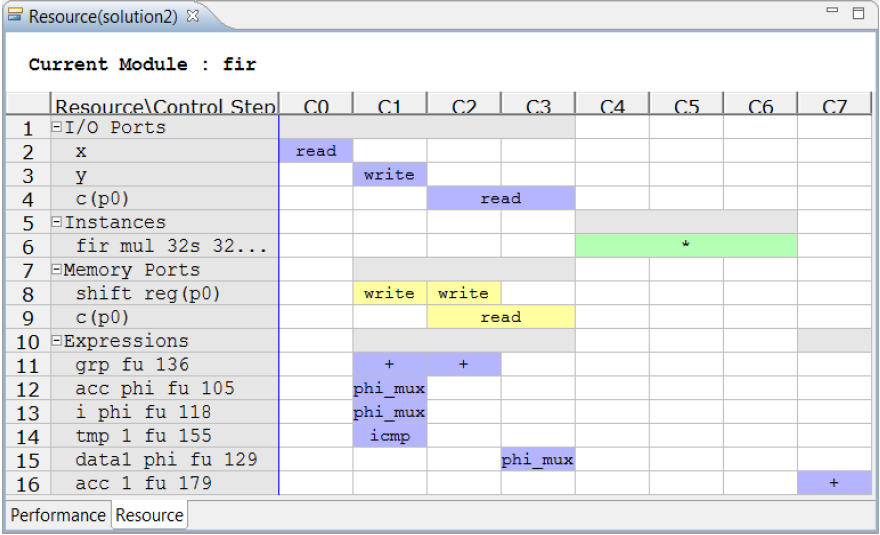
\includegraphics[scale=0.7]{img/Resource.png} 
    \end{center}
\end{minipage}
\begin{center}
Multiplikationsformel
\end{center}

\subsection {die benötigten Operationen des Design und deren Laufzeit}
In der linken Feld der Performance\-Ansicht werden die Operationen im Modul der RTL\-Hierarchie angezeigt.\\



\section{Aufgabe 2} \label{ex2}
In der Aufgabe 2 wurde eine Fibonacci-Algorithm in c mitgebracht. Der Code wurde mit HLS synthetisiert und sowohl den Ressourcenverbrauch als auch das Timing unseres Codes analysiert.

\subsection{C-Code}
C-Code zur Berechnung des n-ten Wertes F(n) der  Fibonacci-Folge aus den Startwerten F0 = 0 und F1 = 1\\

Fibonacci für Hardware Implementation
\begin{verbatim}
#include "fir.h"

void fir (
  data_t result[20],
  data_t n
  ) {

  int i;
  *result = 0;
  *(result+1) = 1;
  Shift_Accum_Loop: for (i=2;i<20;i++) {
	  *(result+i) =  *(result+i-1) +  *(result+i-2);
  }
}
\end{verbatim}

Testbench
\begin{verbatim}
#include <stdio.h>
#include <math.h>
#include "fir.h"

int main () {
   FILE         *fp;

  data_t signal, output[N];
  //coef_t taps[N] = {2,100,9};

  int i;
  
  fp=fopen("out.dat","w");
  fir(output,N);

  for (i=0;i<N;i++) {
	// Execute the function with latest input
	// Save the results.
    fprintf(fp," the %d-Fibonatchi is =  %d\n",i+1,output[i]);
  }
  fclose(fp);

  printf ("Comparing against output data \n");
  if (system("diff -w out.dat out.gold.dat")) {

	fprintf(stdout, "*******************************************\n");
	fprintf(stdout, "FAIL: The result is not correct\n");
	fprintf(stdout, "*******************************************\n");
     return 1;
  } else {
	fprintf(stdout, "*******************************************\n");
	fprintf(stdout, "PASS: The result is correct!\n");
	fprintf(stdout, "*******************************************\n");
     return 0;
  }
}
\end{verbatim}

\subsection{C-Code Analyse}
Das Bild zeigt den Ressourcenverbrauch und das Timing\\

\begin{minipage}{\textwidth}
    \begin{center}        
        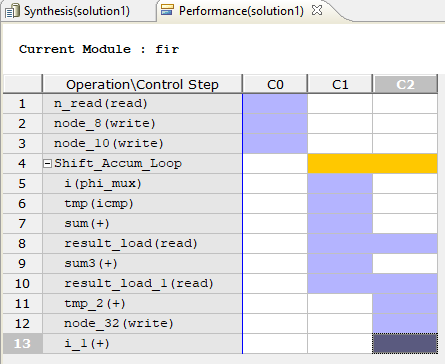
\includegraphics[scale=0.75]{img/Fibo.png} 
    \end{center}
\end{minipage}
\begin{center}
Perfomance in Zyklen
\end{center}

\begin{minipage}{\textwidth}
    \begin{center}        
        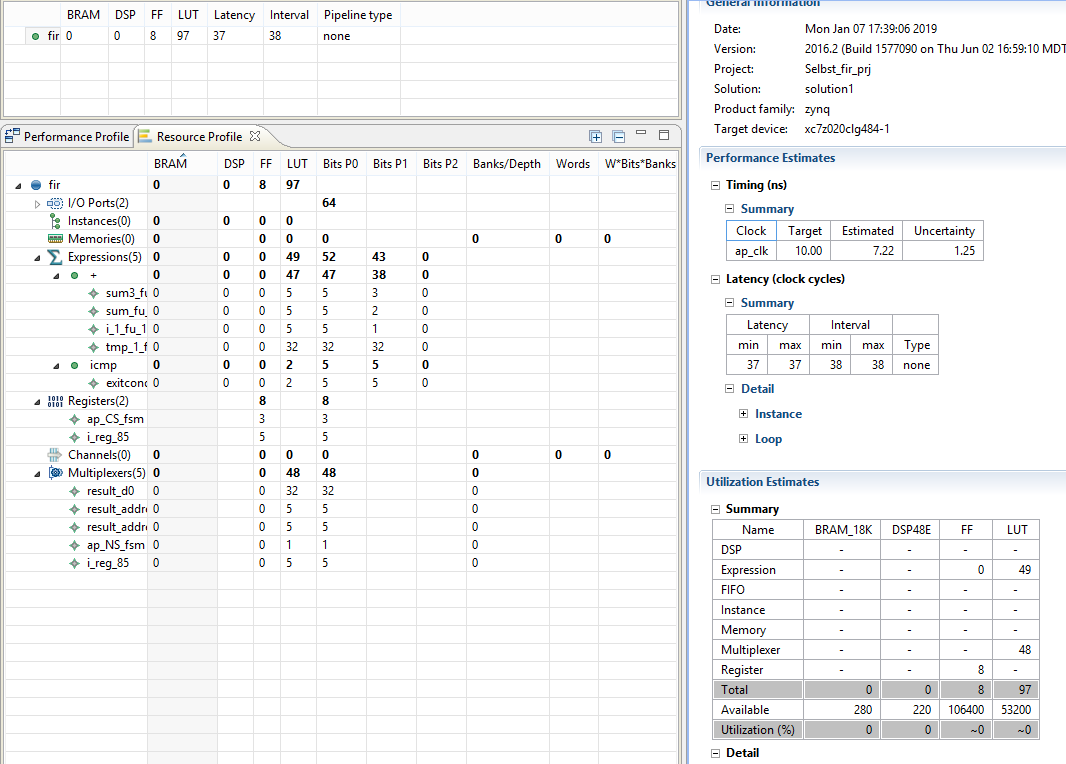
\includegraphics[scale=0.6]{img/fibo1.png} 
    \end{center}
\end{minipage}
\begin{center}
Ressourcenverbrauch 1
\end{center}

\begin{minipage}{\textwidth}
    \begin{center}        
        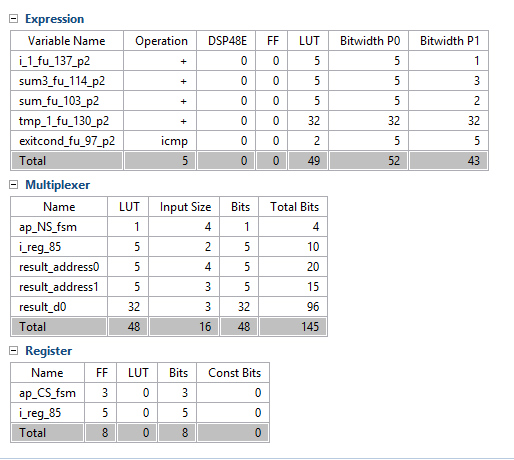
\includegraphics[scale=1.0]{img/fibo2.png} 
    \end{center}
\end{minipage}
\begin{center}
Ressourcenverbrauch 2
\end{center}







\end{document}
